% !TeX root = ../main.tex
\section{模型建立与求解}

\subsection{问题一：抽样检测方案}

本问以一批零配件的真实次品率 $p$ 为待判断参数，以预先固定的抽样数 $n$ 和样本次品数 $X$ 为观测对象。题目未给出批次总量 $N$、不可接受次品率与目标检验功效，因此本文以二项模型给出数值结论，超几何分布仅在已知 $N$ 且无放回抽样时作为有限总体修正；样本量与判定阈值在观察数据前确定，同一固定样本方案只实施一次，所得样本量不解释为传统功效分析样本量。

\subsubsection{精确单侧检验与三态判定}

对拒收结论建立单侧假设
\begin{equation}
  H_{0R}:p\le p_0,\qquad H_{1R}:p>p_0,
  \label{eq:q1-reject-hypothesis}
\end{equation}
并令拒收显著性水平为 $\alpha_R=1-\gamma_R=0.05$。对接收结论建立反向单侧假设
\begin{equation}
  H_{0A}:p\ge p_0,\qquad H_{1A}:p<p_0,
  \label{eq:q1-accept-hypothesis}
\end{equation}
相应显著性水平为 $\alpha_A=1-\gamma_A=0.10$。

两个检验分别控制错拒合格批和错收不合格批的概率。离散样本不一定能在给定显著性水平下支持任一方向的结论，因此保留中间的证据不足区域。对给定 $n$，若接收临界值为 $a_n$、拒收临界值为 $r_n$，则
\begin{equation}
  \operatorname{Decision}(x)=
  \begin{cases}
    \text{接收}, & x\le a_n,\\
    \text{证据不足}, & a_n<x<r_n,\\
    \text{拒收}, & x\ge r_n.
  \end{cases}
  \label{eq:q1-three-way-decision}
\end{equation}
其中 $a_n<r_n$，从而保证接收域与拒收域互不重叠。

\subsubsection{二项分布抽样模型}

在总体量未知或抽样比例较小时，将每件零配件视为一次独立伯努利试验。在边界 $p=p_0$ 上，样本次品数满足
\begin{equation}
  X\sim\operatorname{Bin}(n,p_0),\qquad
  P(X=k)=\binom{n}{k}p_0^k(1-p_0)^{n-k}.
  \label{eq:q1-binomial-pmf}
\end{equation}
二项精确检验与超几何有限总体检验属于经典数理统计方法\cite{stat-casella}。

式~\eqref{eq:q1-reject-hypothesis}中的右尾概率随 $p$ 增大，复合原假设的最不利点为 $p=p_0$，故拒收临界值为
\begin{equation}
  r_n=\min\left\{x:
  \sum_{k=x}^{n}\binom{n}{k}p_0^k(1-p_0)^{n-k}
  \le \alpha_R\right\}.
  \label{eq:q1-binomial-reject-cutoff}
\end{equation}
式~\eqref{eq:q1-accept-hypothesis}中的左尾概率在 $p=p_0$ 处达到原假设范围内的最大值，故接收临界值为
\begin{equation}
  a_n=\max\left\{x:
  \sum_{k=0}^{x}\binom{n}{k}p_0^k(1-p_0)^{n-k}
  \le \alpha_A\right\}.
  \label{eq:q1-binomial-accept-cutoff}
\end{equation}

\subsubsection{有限总体修正}

当批次总量 $N$ 已知且采用无放回抽样时，抽取一个样品会改变剩余总体组成。令总体中的实际次品数为 $D$，则
\begin{equation}
  P(X=k\mid N,D,n)
  =\frac{\binom{D}{k}\binom{N-D}{n-k}}{\binom{N}{n}}.
  \label{eq:q1-hypergeometric-pmf}
\end{equation}
为对应“总体次品率不超过标称值”，定义
\begin{equation}
  D_0=\lfloor Np_0\rfloor,\qquad D_1=D_0+1,
  \label{eq:q1-finite-boundaries}
\end{equation}
其中 $D_0$ 是最大可接受次品数，$D_1$ 是最小不可接受次品数。拒收方向以 $D_0$ 控制错拒概率，接收方向以 $D_1$ 控制错收概率，得到
\begin{align}
  r_{n,N}
  &=\min\{x:P(X\ge x\mid N,D_0,n)\le\alpha_R\},
  \label{eq:q1-hyper-reject}\\
  a_{n,N}
  &=\max\{x:P(X\le x\mid N,D_1,n)\le\alpha_A\}.
  \label{eq:q1-hyper-accept}
\end{align}
这两个边界与二项模型共用三态判定结构，仅把独立抽样概率替换为无放回抽样概率；当 $n=N$ 时退化为全检判定，该性质同时用于检验程序实现。

\subsubsection{最小样本量与判定方案}

“检测次数尽可能少”需要可计算的操作化口径。仅要求某个极端结果能够触发拒收时，很小样本量即可满足尾概率约束，但该方案不能同时给出接收域，也不能识别轻度超标批次。为使一个固定样本方案同时具备可执行的接收与拒收能力，本文以“同一 $n$ 下接收域与拒收域均非空且互不重叠”作为主要最小性准则，并同时报告两种方向性口径：
\begin{equation}
  n_R=\min\{n:r_n\text{ 存在}\},\qquad
  n_A=\min\{n:a_n\text{ 存在}\},
  \label{eq:q1-min-directional-n}
\end{equation}
以及统一样本量
\begin{equation}
  n_*=\min\{n:a_n\text{ 与 }r_n\text{ 同时存在且 }a_n<r_n\}.
  \label{eq:q1-min-unified-n}
\end{equation}

在拒收方向，最有利的极端结果为 $x=n$，其右尾概率为 $p_0^n$。由 $0.1^n\le0.05$ 得 $n_R=2$，这只表示抽取两件且两件均为次品时可以拒收，不代表该小样本方案对一般超标批次具有较高检验功效。在接收方向，最有利的结果为 $x=0$，由
\[
  0.9^n\le0.10,\qquad
  n\ge\frac{\ln0.10}{\ln0.90}=21.854\cdots,
\]
得 $n_A=22$。当 $n=22$ 时拒收域也已存在且两类判定域不重叠，故 $n_*=22$，三种口径见表~\ref{tab:q1-minimum-samples}。

\begin{table}[H]
  \centering
  \caption{不同口径下的最小样本量}
  \label{tab:q1-minimum-samples}
  \begin{tabular}{p{0.27\textwidth}cp{0.43\textwidth}}
    \toprule
    口径 & 最小样本量 & 首次可触发的样本结果 \\
    \midrule
    首次存在拒收域 & $n_R=2$ & $x=2$ 时拒收 \\
    首次存在接收域 & $n_A=22$ & $x=0$ 时接收 \\
    首次同时存在两个判定域 & $n_*=22$ & $x=0$ 接收，$x\ge6$ 拒收 \\
    \bottomrule
  \end{tabular}
\end{table}

程序以 $p_0=0.10$、$\gamma_R=0.95$、$\gamma_A=0.90$ 为参数，在 $n=1,2,\ldots,200$ 上顺序枚举：对每个 $n$ 在对数域生成并归一化二项或超几何概率，构造左右尾累积概率，搜索最大的接收临界值与最小的拒收临界值，并检查临界点、相邻点及判定域不重叠约束；该过程为确定性精确枚举，不使用随机数。由此得到固定样本方案：随机抽取 $22$ 件并完成检测，判定规则为
\begin{equation}
  \operatorname{Decision}(x)=
  \begin{cases}
    \text{接收该批}, & x=0,\\
    \text{证据不足}, & 1\le x\le5,\\
    \text{拒收该批}, & x\ge6.
  \end{cases}
  \label{eq:q1-final-binomial-rule}
\end{equation}

\subsubsection{结果分析与敏感性检验}

表~\ref{tab:q1-boundary-check}给出 $n=22$ 时的临界概率及相邻点概率：接收临界点满足 $P(X\le0)<0.10$，增加一个次品后左尾概率立即超过 $0.10$；拒收临界点满足 $P(X\ge6)<0.05$，减少一个次品后右尾概率超过 $0.05$。因此 $a_{22}=0$ 是最大接收临界值，$r_{22}=6$ 是最小拒收临界值。

\begin{table}[H]
  \centering
  \caption{$n=22$ 时二项模型的临界概率校核}
  \label{tab:q1-boundary-check}
  \begin{tabular}{p{0.38\textwidth}ccc}
    \toprule
    校核量 & 概率 & 约束 & 结论 \\
    \midrule
    $P(X\le0)$ & $0.0984770902$ & $\le0.10$ & 通过 \\
    $P(X\le1)$ & $0.3391988663$ & $>0.10$ & 相邻点不接收 \\
    $P(X\ge6)$ & $0.0182159811$ & $\le0.05$ & 通过 \\
    $P(X\ge5)$ & $0.0621336713$ & $>0.05$ & 相邻点不拒收 \\
    \bottomrule
  \end{tabular}
\end{table}

图~\ref{fig:q1-decision-boundaries}给出样本量变化时两个临界值的相对位置：接收上界始终位于拒收下界之下，两条曲线之间为证据不足区；对 $n=1,2,\ldots,200$ 的枚举结果复核表明，所有临界点均满足相应尾概率约束且判定域不重叠。

\begin{figure}[H]
  \centering
  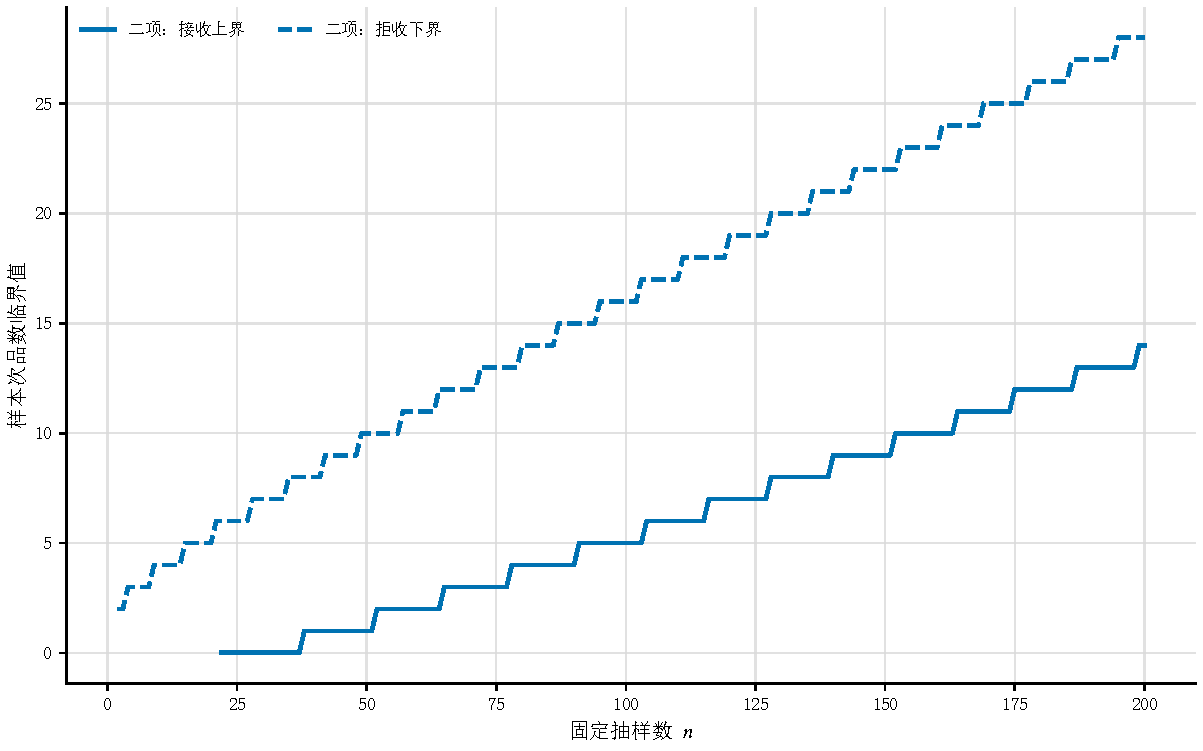
\includegraphics[width=0.90\textwidth]{../../figures/q1/q1_decision_boundaries.pdf}
  \caption{二项模型的接收与拒收临界值随样本量的变化}
  \label{fig:q1-decision-boundaries}
\end{figure}

有限总体分支以 $N=1000$ 作性质校核：此时 $D_0=100$、$D_1=101$，计算得到 $n_*=22$、$a_{22,1000}=0$、$r_{22,1000}=6$，临界概率为 $P_{D_1}(X\le0)=0.0935984699$、$P_{D_0}(X\ge6)=0.0170168477$，相邻点概率 $0.3304729576$ 与 $0.0600260183$ 仍满足临界值极值性。该组数值只用于验证超几何计算性质；实际 $N$ 一旦获得，应按式~\eqref{eq:q1-hyper-reject}和式~\eqref{eq:q1-hyper-accept}重新计算。

问题一的主要风险有两类：结论可能对置信水平敏感，以及小总体下二项近似可能偏离无放回抽样。为此分别进行单因素置信水平扰动和有限总体情景分析，改变一个置信水平时保持 $p_0=0.10$ 及另一置信水平为题目给定值，观察相应方向首次存在判定域的样本量；改变 $N$ 时保持两类信度不变，观察统一样本量 $n_*$。本节所有 $N$ 均为检验网格，不是题面数据。

表~\ref{tab:q1-confidence-sensitivity}与图~\ref{fig:q1-confidence-sensitivity}给出置信水平扰动结果。接收信度由 $0.80$ 提高到 $0.99$ 时，首次能够接收的样本量由 $16$ 增至 $44$，说明接收侧样本量对置信水平较敏感；接收方向需要用很少的次品数排除 $p\ge p_0$ 的情形，信度越高，必须积累越多无次品证据。拒收方向的方向性样本量变化较小，是因为该指标只要求存在一个极端拒收结果，并不衡量一般不合格批次的检验功效，不能把 $n_R=1$ 或 $2$ 单独解释为充分的统一方案。

\begin{table}[H]
  \centering
  \caption{置信水平对方向性最小样本量的影响}
  \label{tab:q1-confidence-sensitivity}
  \begin{tabular}{cccc}
    \toprule
    拒收信度 & 首次拒收样本量 & 接收信度 & 首次接收样本量 \\
    \midrule
    $0.900$ & $1$ & $0.80$ & $16$ \\
    $0.925$ & $2$ & $0.85$ & $19$ \\
    $0.950$ & $2$ & $0.90$ & $22$ \\
    $0.975$ & $2$ & $0.95$ & $29$ \\
    $0.990$ & $2$ & $0.99$ & $44$ \\
    \bottomrule
  \end{tabular}
\end{table}

\begin{figure}[H]
  \centering
  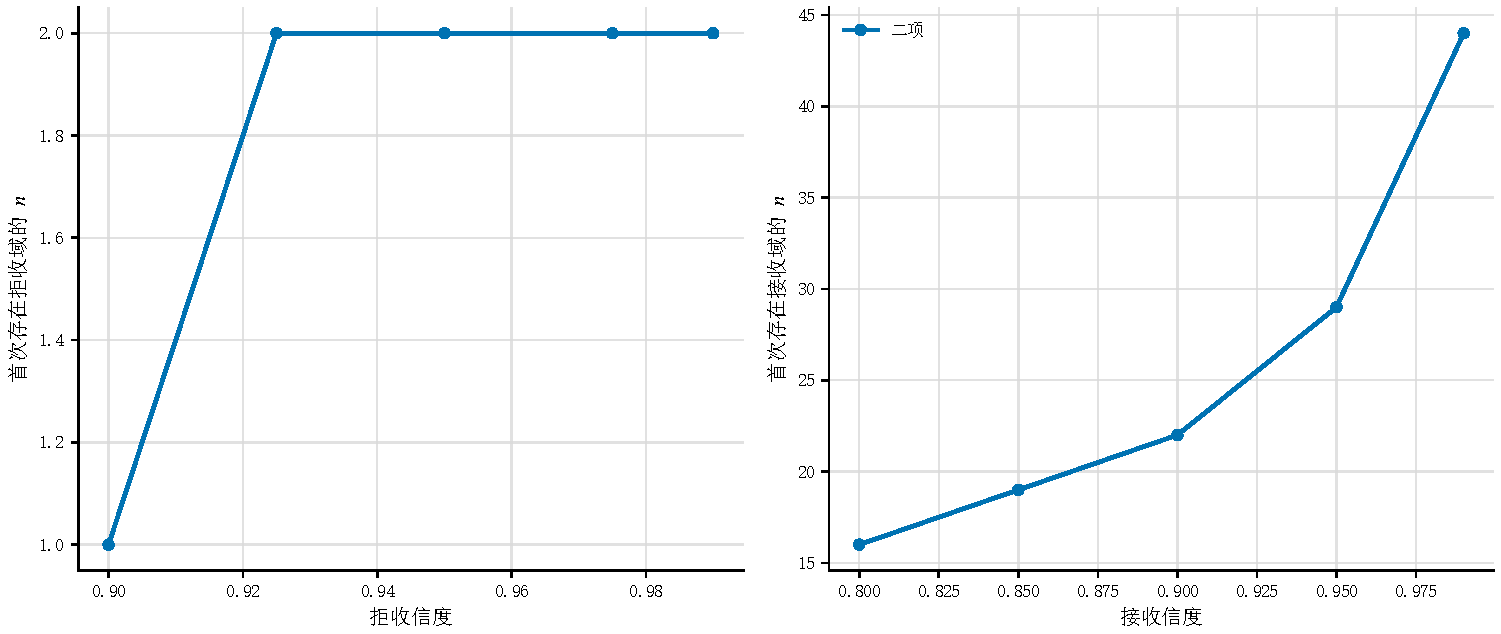
\includegraphics[width=0.96\textwidth]{../../figures/q1/q1_confidence_sensitivity.pdf}
  \caption{置信水平变化对方向性最小样本量的影响}
  \label{fig:q1-confidence-sensitivity}
\end{figure}

表~\ref{tab:q1-population-sensitivity}与图~\ref{fig:q1-population-sensitivity}比较不同有限总体量下的超几何统一样本量及二项极限。总体量较小时，抽样占总体的比例较高，无放回抽样提供了更多总体组成信息，所需样本量小于二项模型结果；随着 $N$ 增大，有限总体修正逐渐减弱，当 $N=1000$ 和 $5000$ 时本组参数下 $n_*=22$，与二项模型一致。该趋势支持在总体量较大或抽样比例较低时使用二项模型，而小批次应优先采用超几何精确计算。

\begin{table}[H]
  \centering
  \caption{有限总体量对超几何统一样本量的影响}
  \label{tab:q1-population-sensitivity}
  \begin{tabular}{rrrr}
    \toprule
    $N$ & $D_0=\lfloor0.1N\rfloor$ & 超几何模型 $n_*$ & 相对二项模型差值 \\
    \midrule
    $25$ & $2$ & $13$ & $-9$ \\
    $50$ & $5$ & $16$ & $-6$ \\
    $100$ & $10$ & $18$ & $-4$ \\
    $200$ & $20$ & $20$ & $-2$ \\
    $500$ & $50$ & $21$ & $-1$ \\
    $1000$ & $100$ & $22$ & $0$ \\
    $5000$ & $500$ & $22$ & $0$ \\
    \bottomrule
  \end{tabular}
\end{table}

\begin{figure}[H]
  \centering
  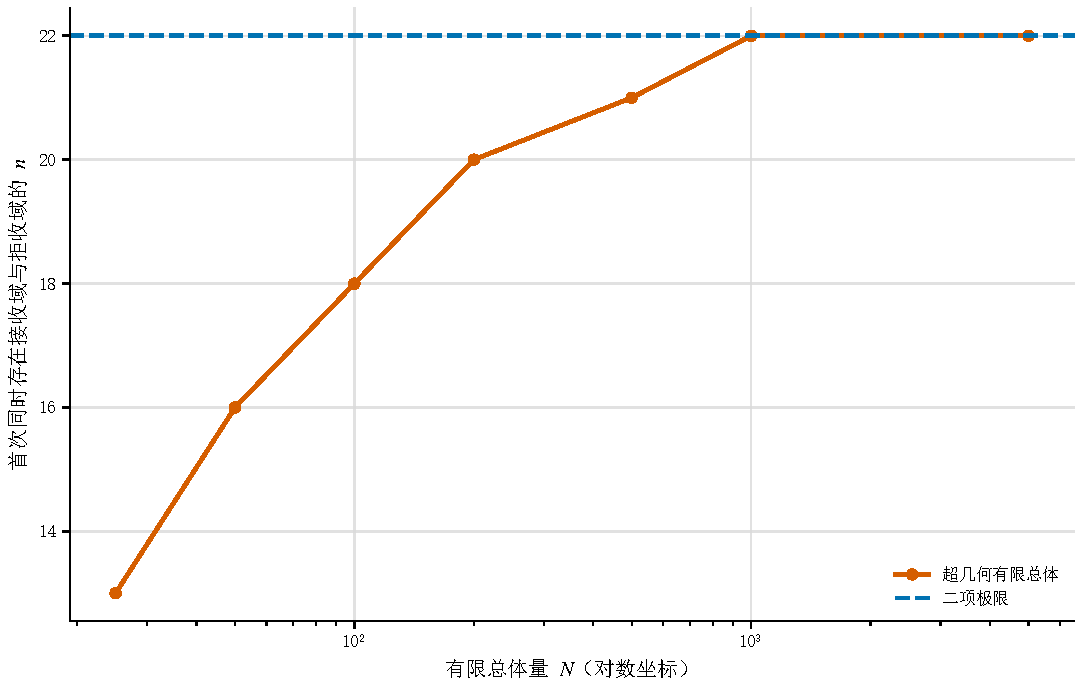
\includegraphics[width=0.88\textwidth]{../../figures/q1/q1_population_sensitivity.pdf}
  \caption{有限总体量变化下超几何模型与二项极限的比较}
  \label{fig:q1-population-sensitivity}
\end{figure}

两组检验表明：统一方案中的接收侧样本量会随置信要求明显变化，改变信度后应重新计算，不能继续沿用 $n=22$；有限总体量增大时，超几何结果收敛到二项结果。无论采用何种参数，样本量和临界值均应在抽样前确定，并保留证据不足区域。上述结论限定在给定参数网格内。

\subsubsection{本问结论}

在 $10\%$ 标称次品率、$95\%$ 拒收信度和 $90\%$ 接收信度下，统一方案为抽取 $22$ 件：未发现次品时接收，发现不少于 $6$ 个次品时拒收，发现 $1$ 至 $5$ 个次品时保留为证据不足。该方案适用于总体量未知或抽样比例较小的固定样本场景；小批量无放回抽样应输入实际 $N$ 后采用超几何修正。该批次判断及其不确定区为后续生产决策提供质量信息边界。
